\begin{frame}{Расчёт ЛТХ}
\begin{block}{В расчёт ЛТХ входит}
   \begin{enumerate}
    \item [] <+->
    \item <+-> Расчёт области возможных полётов
    \item <+-> Расчёт траектории полёта 
    \item <+-> Расчёт транспортных возможностей самолёта
   \end{enumerate}
\end{block}
\end{frame}

\begin{frame}{Расчёт ЛТХ}{Расчёт области возможных полётов}

    \begin{block}{Основные ограничения}
        \begin{itemize}
            \item Ограничение по $M_{min \ P}$ 
            \item Ограничение по $M_{max \ P}$
        \end{itemize}
    \end{block}

    \begin{block}{Дополнительные ограничения}
        \begin{itemize}
            \item Ограничение по $C_{y \ \text{доп}}$
            \item Ограничение по $M_\text{пред}$
            \item Ограничение по $q_{max}$
        \end{itemize}
    \end{block}

\end{frame}

\begin{frame}{Расчёт ЛТХ}{Результаты расчётов $M_{C_{y \ \text{доп}}}$ и $M_{min \ P}$, $M_{max \ P}$, $M_\text{наев}$}
    \begin{minipage}[c]{0.45\textwidth}
        \center{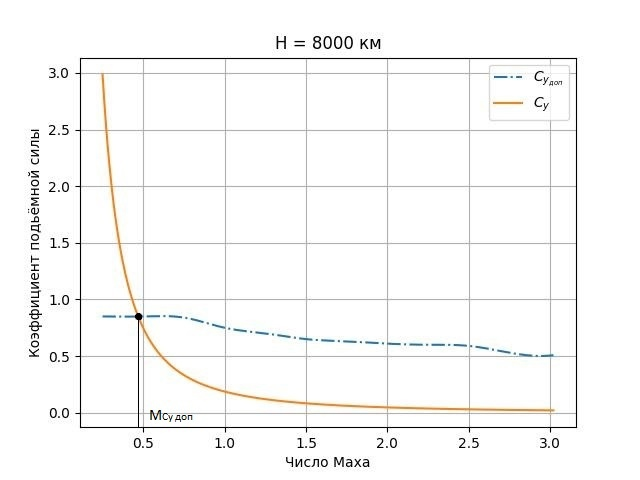
\includegraphics[width=6cm, height = 7cm]{../Оглавление/Part1/figures/CyCydop2.jpg}}
    \end{minipage}
    \begin{minipage}[c]{0.45\textwidth}
        \center{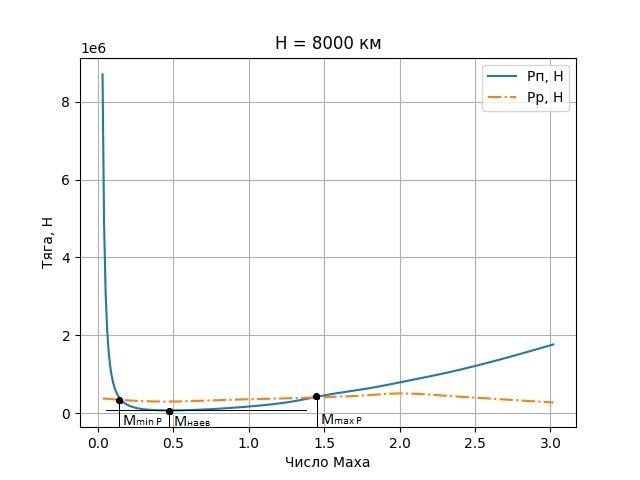
\includegraphics[width=6cm, height = 7cm]{../Оглавление/Part1/figures/PpPr2.jpg}}
    \end{minipage}
\end{frame}

\begin{frame}{Расчёт ЛТХ}{Результаты расчётов $q_{\text{ч} \ min}$ и $q_{\text{км} \ min}$}
    \begin{minipage}[c]{0.45\textwidth}
        \center{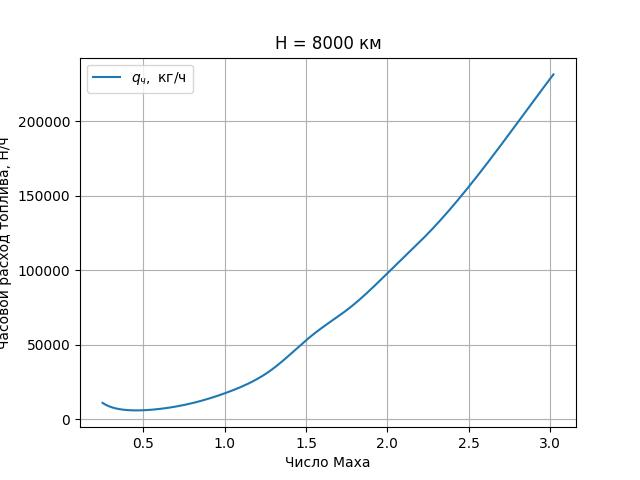
\includegraphics[width=6cm, height = 7cm]{../Оглавление/Part1/figures/qh2.jpg}}
    \end{minipage}
    \begin{minipage}[c]{0.45\textwidth}
        \center{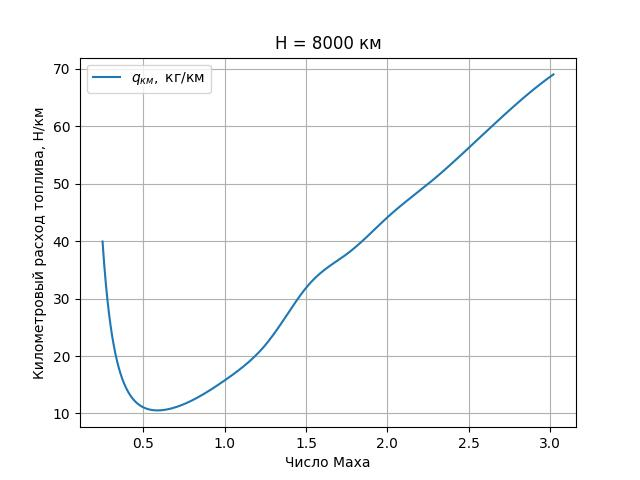
\includegraphics[width=6cm, height = 7cm]{../Оглавление/Part1/figures/qkm2.jpg}}
    \end{minipage}
\end{frame}

\begin{frame}{Расчёт ЛТХ}{Результаты расчётов $M_{V_{y \ max}}$}
        \center{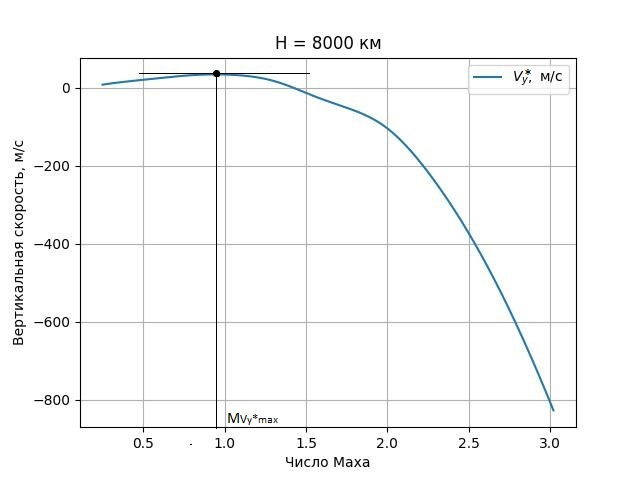
\includegraphics[width=10cm, height = 7cm]{../Оглавление/Part1/figures/Vy2.jpg}}
\end{frame}

\begin{frame}{Расчёт ЛТХ}{Расчёт области возможных полётов}
    \begin{minipage}[c]{0.55\textwidth}
        \center{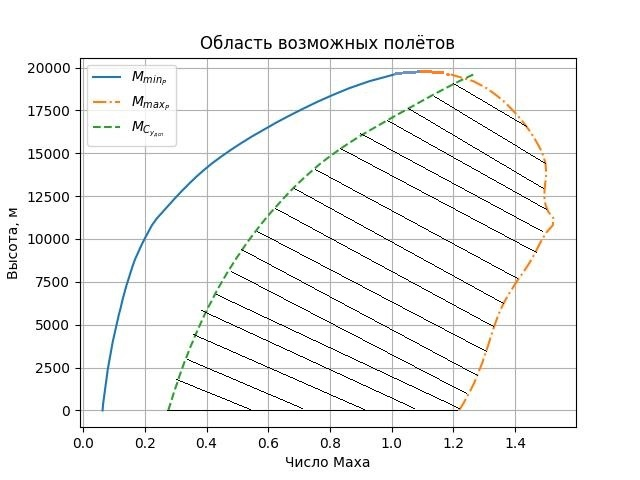
\includegraphics[width=6cm, height = 7cm]{../Оглавление/Part1/figures/Область.jpg}}
    \end{minipage}
    \begin{minipage}[c]{0.4\textwidth}
        \begin{itemize}
            \item <+-> []
            \item <+-> [] \begin{block}{Определение области}
                \begin{itemize}
                    \item $M_{min} = max \{ M_{min \ p}, \ M_{C_{y \ \text{доп}}} \} $
                    \item $M_{max} = min \{ M_{max \ P}, \ M_{\text{пред}}, \ M_{q_{max}} \}$
                \end{itemize}
            \end{block}
        \end{itemize}
    \end{minipage}
\end{frame}

\begin{frame}{Расчёт ЛТХ}{Определение теоретического и практического потолка}
    \begin{minipage}[c]{0.45\textwidth}
        \begin{block}{Потолки}
        \begin{itemize}
            \item <+-> []
            \item <+-> [] Расчёт теоретического и практического потолка производится по $V^*_{y_{max}}$
            \item <+-> [] $H_\text{т} = 19,8$ км 
            \item <+-> [] $H_\text{пр} = 19,5$ км
        \end{itemize}
        \end{block}
    \end{minipage}
    \begin{minipage}[c]{0.45\textwidth}
        \center{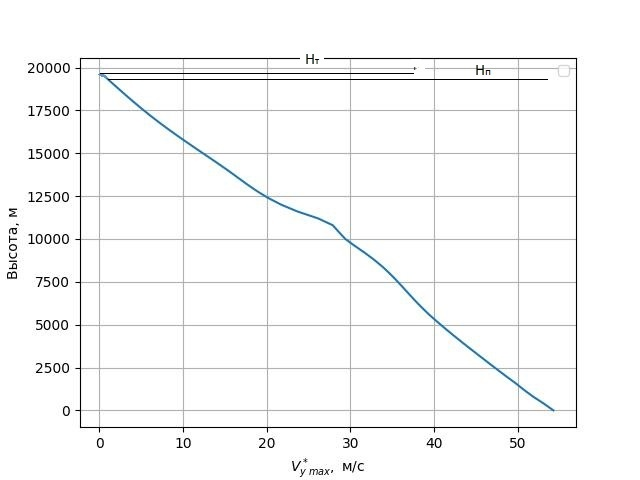
\includegraphics[width=6cm, height = 7cm]{../Оглавление/Part1/figures/Vy(H).jpg}}
    \end{minipage}
\end{frame}

\begin{frame}{Расчёт ЛТХ}{Максимальные значения часового и километрового расходов}
        \center{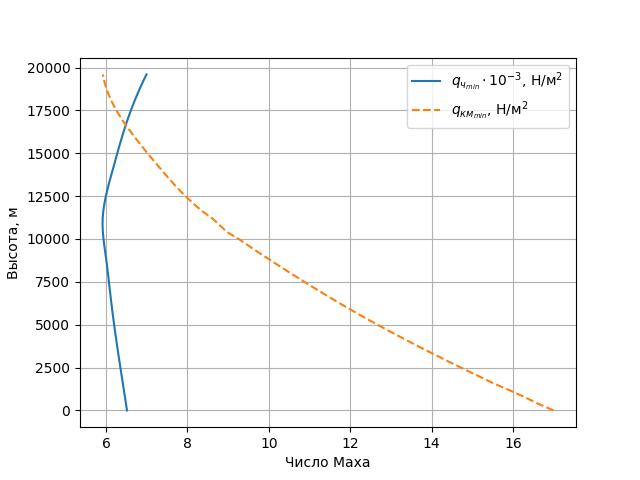
\includegraphics[width=10cm, height = 7cm]{../Оглавление/Part1/figures/qhqkm_MAX.jpg}}
\end{frame}

\begin{frame}{Расчёт ЛТХ}{Расчёт траектории полёта}
    \begin{block}{Траектория}
    \begin{itemize}
        \item [] <+->
        \item [] <+-> Траеткорию полёта принято разделять на три этапа 
            \begin{itemize}
                \item Набор высоты 
                \item Крейсерский полёт 
                \item Снижение 
            \end{itemize}
    \end{itemize}
    \end{block}
\end{frame}

\begin{frame}{Расчёт ЛТХ}{Расчёт траектории набора}
    \begin{block}{Выбор начальных параметров}
        Начальные значения H и М определяются следующим образом: $H_0$ = 0 км $M_0$ = 1,2$\cdot M_{min \ \text{доп}}$, а конечные значения выбираются из
        условия минимума километрового расхода топлива в установившемся горизонтальном полете. Высота и число Маха, при которых километровый расход 
        топлива принимает наименьшее значение, определены в предыдущих слайдах 
    \end{block}
\end{frame}

\begin{frame}{Расчёт ЛТХ}{Расчёт траектории набор}
    \begin{minipage}[c]{0.45\textwidth}
        \center{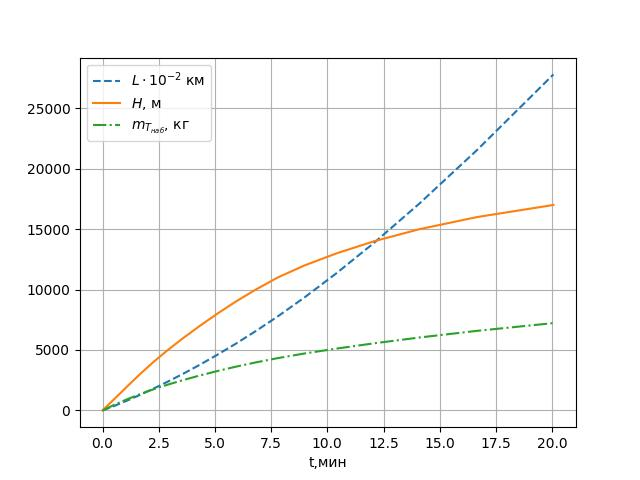
\includegraphics[width=6cm, height = 7cm]{../Оглавление/Part1/figures/Характеристики набора высоты1.jpg}}
    \end{minipage}
    \begin{minipage}[c]{0.45\textwidth}
        \center{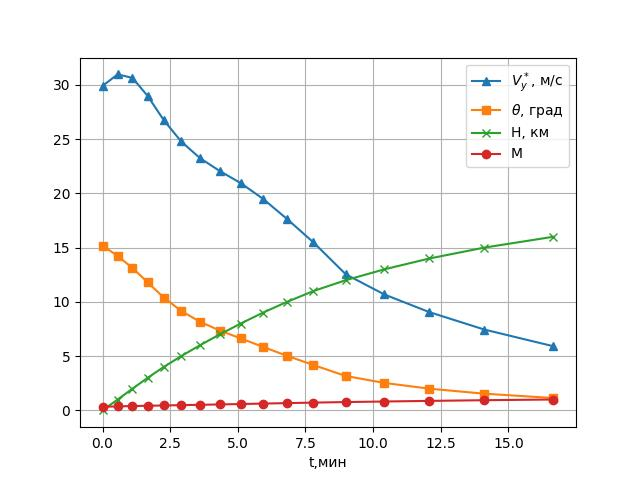
\includegraphics[width=6cm, height = 7cm]{../Оглавление/Part1/figures/Характеристики набора высоты2.jpg}}
    \end{minipage}
\end{frame}
 
\begin{frame}{Расчёт ЛТХ}{Расчёт траектории набора}
    \begin{block}{Результаты расчётов}
    \begin{table}
        \begin{tabular}{|c|c|c|}
            \hline
            Параметр&  Значение & Единицы  \\ \hline
            $m_{T_{\text{наб}}}$& 7225,6 &кг \\ \hline
            $L_\text{наб}$& 278,04 &км \\ \hline
            $T_\text{наб}$& 20,06 & мин\\ \hline
        \end{tabular}
    \end{table}
    \end{block}
\end{frame}

\begin{frame}{Расчёт ЛТХ}{Расчёт крейсерского полёта}
    \begin{block}{Выбор начальных параметров}
        $\bar{m}_{T_\text{наб}}$ = 0,5 – относительная масса пустого снаряженного самолета \\ 
        $\bar{m}_\text{цн}$ = 0,15 – относительная масса целевой нагрузки \\ 
        $\bar{m}_\text{снп}$ = 0,015 – относительная масса топлива 
        расходуемая при снижении и посадке  \\
        $\bar{m}_{T_\text{наб}}$– относительная масса топлива, расходуемая при наборе высоты \\
    \end{block}
    \begin{itemize}
        \item <+-> []
    \item <+-> [] \begin{block}{Результаты расчётов характеристик крейсерского полёта}
        \begin{table}
            \begin{tabular}{|c|c|c|}
                \hline
                Параметр& Значение & Единицы\\ \hline
                $H_\text{к \ кр}$& 19.3 & км\\ \hline
                $L_\text{кр}$& 7610,74 &кг \\ \hline
                $T_\text{кр}$& 403,43 & мин\\ \hline
            \end{tabular}
        \end{table}
    \end{block}
    \end{itemize}
\end{frame} 

\begin{frame}{Расчёт ЛТХ}{Расчёт траектории спуска} %Предупреждение
        \begin{minipage}[c]{0.45\textwidth}
            \center{\includegraphics[width=6cm, height = 7cm]{../Оглавление/Part1/figures/Характеристики спуска1.jpg}}
        \end{minipage}
        \begin{minipage}[c]{0.45\textwidth}
            \center{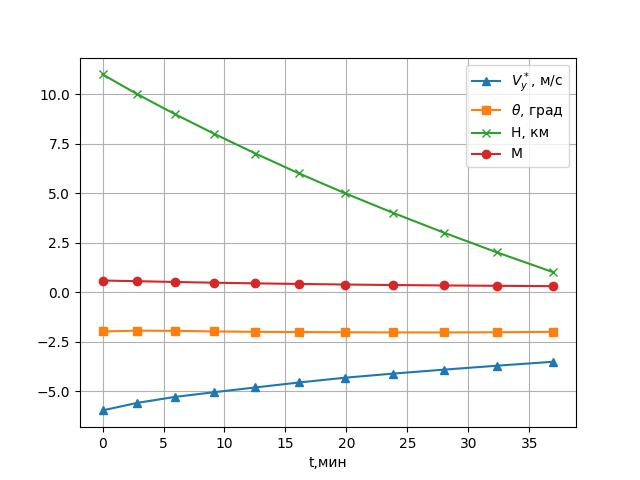
\includegraphics[width=6cm, height = 7cm]{../Оглавление/Part1/figures/Характеристики пуска2.jpg}}
        \end{minipage}
\end{frame}

\begin{frame}{Расчёт ЛТХ}{Расчёт траектории спуска}
    \begin{block}{Результаты расчётов}
        \begin{table}
            \begin{tabular}{|c|c|c|}
                \hline
                Параметр& Значение & Единицы\\ \hline
                $m_{T_\text{спуск}}$&756,936 & кг\\ \hline
                $L_\text{спуск}$& 314,16 &км \\ \hline
                $T_\text{спусе}$& 41,929 & мин\\ \hline
            \end{tabular}
        \end{table}
    \end{block}
\end{frame}

\begin{frame}{Расчёт ЛТХ}{Расчёт траектории полёта}
    \center{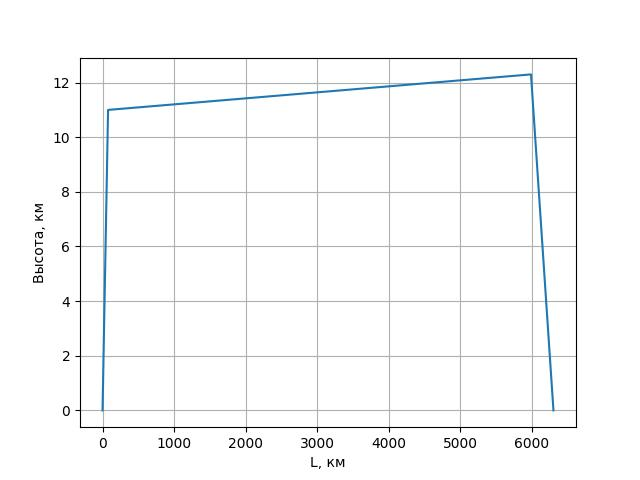
\includegraphics[width=10cm, height = 8cm]{../Оглавление/Part1/figures/Траектория полета.jpg}}
\end{frame}

\begin{frame}{Расчёт ЛТХ}{Расчёт транспортных возможностей самолёта}
    \begin{itemize}
        \item <+-> []
        \item <+-> [] \begin{block}{Основные положения}
            \begin{itemize}
            \item <+-> [] Расчёт ведётся для трёх режимов
            \begin{itemize}
                \item <+-> Полет с максимальной коммерческой нагрузкой
                \item <+-> Полёт с максимальным запасом топлива
                \item <+-> Полёт без коммерческой нагрузки ($m_\text{цн}$ = 0) с максимальным запасом топлива
            \end{itemize}
        \end{itemize}
        \end{block}
    \end{itemize}
\end{frame}

\begin{frame}{Расчёт ЛТХ}{Диаграмма транспортных возможностей самолёта}
    \center{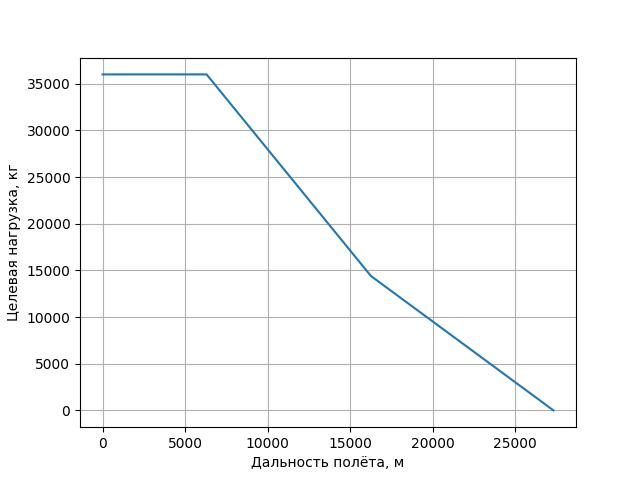
\includegraphics[width=10cm, height = 8cm]{../Оглавление/Part1/figures/Транспортные возможности.jpg}}
\end{frame}